\documentclass{article}
\usepackage{tikz}
\usetikzlibrary{arrows.meta,positioning,calc,shapes.geometric}
\pagestyle{empty}
\begin{document}
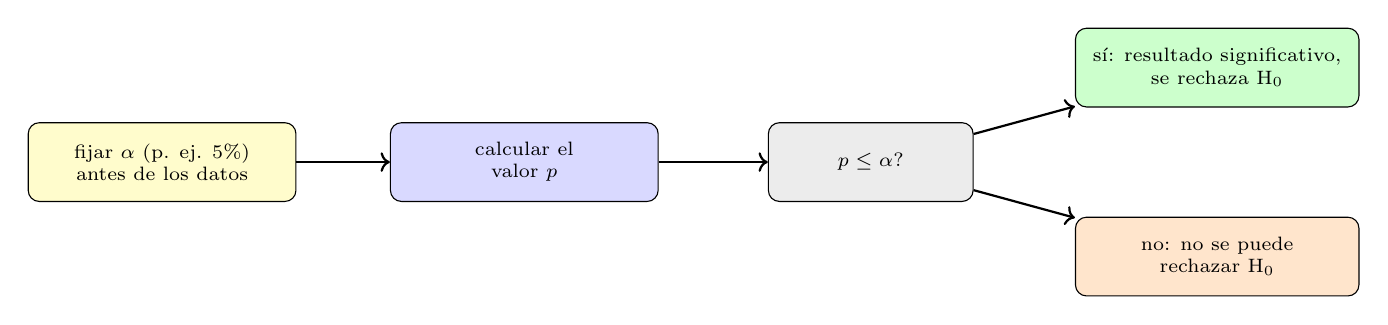
\begin{tikzpicture}
\tikzset{every node/.append style={align=center}}

\node[draw, rounded corners, fill=yellow!20, minimum width=3.4cm, minimum height=1.0cm, align=center, font=\scriptsize] (a) at (0,0) {fijar $\alpha$ (p. ej. 5\%)\\ antes de los datos};
\node[draw, rounded corners, fill=blue!15, minimum width=3.4cm, minimum height=1.0cm, align=center, font=\scriptsize] (b) at (4.6,0) {calcular el\\ valor $p$};
\node[draw, rounded corners, fill=gray!15, minimum width=2.6cm, minimum height=1.0cm, align=center, font=\scriptsize] (c) at (9.0,0) {$p \le \alpha$?};
\node[draw, rounded corners, fill=green!20, minimum width=3.6cm, minimum height=1.0cm, align=center, font=\scriptsize] (d) at (13.4,1.2) {sí: resultado significativo,\\ se rechaza H$_0$};
\node[draw, rounded corners, fill=orange!20, minimum width=3.6cm, minimum height=1.0cm, align=center, font=\scriptsize] (e) at (13.4,-1.2) {no: no se puede\\ rechazar H$_0$};
\draw[->, thick] (a) -- (b); \draw[->, thick] (b) -- (c); \draw[->, thick] (c) -- (d); \draw[->, thick] (c) -- (e);

\end{tikzpicture}
\end{document}
